\section*{Teoretická část}
Budeme měřit povrchové napětí roztoku lihu při koncentracích od 0 do \SI{100}{\percent} odtrhávací metodou.
Tato metoda spočívá v měření síly potřebné k odtržení tenkého drátku od hladiny měřené kapaliny.
Pokud je drátek dostatečně tenký a má délku $l$, drží ho kapalina na hladině silou \cite{ZFP}
\begin{equation} \label{eq::p0sigma}
P_0=2 \cdot \sigma \cdot l \,,
\end{equation}
kde $\sigma$ je povrchové napětí.

Sílu $P_0$ budeme měřit torzními vahami.
Na jedno rameno zavěsíme rámeček, ve kterém je upevněn drátek (viz obr. \ref{obr::ramecek}), a pod něj položíme kádinku s měřeným roztokem.
Na druhé rameno pověsíme přívažky tak, aby odtržení drátku od hladiny proběhlo v rozsahu ciferníku torzních vah.

\begin{figure}[htbp]
\centering
\includegraphics[width=3cm]{graficos/ramecek}
\caption{Náčrt použitého rámečku, na obrázku je vyznačena délka drátku $l$.}
\label{obr::ramecek}
\end{figure}

Protože na drátek nepůsobí pouze síla způsobená povrchovým napětím, změříme nejdříve sílu $P_1$, při které jsou váhy vyvážené a drátek je těsně pod hladinou kapaliny.
Poté budeme sílu zvětšovat a zároveň snižovat kádinku s roztokem, aby váhy zůstali vyvážené.
Při určité síle $P_2$ se drátek odtrhne.
Sílu $P_0$ určíme jako rozdíl sil $P_2$ a $P_1$.

Lenard \cite{oprava} udává korekci na drátek o poloměru $r$
\begin{equation} \label{eq::lenard}
\sigma = \frac{P_0}{2l} - r\left( \sqrt{\frac{P_0 \varrho g}{l}} - \frac{P_0}{l^2} \right) \,,
\end{equation}
kde $\varrho$ je hustota kapaliny a $g$ je tíhové zrychlení.